\chapter{Methods}\label{chap:methods}
\todo{write methods introduction}
{\color{blue}
Chapter on tools (language models) used. What exactly do I want to explain?
First, a bit on how they work in general, second a bit of background on the models, a bit of a comparison (architecture and benchmarks?)
}

% background is more general, methods is specific to the methods we use, in our case LLMs

\section{Language Model Basics}\label{sec:lm}
This Section aims to provide an overview and fundamental understanding of the underlying concepts and terminology of the language models used in this work.
The models part of the benchmark are introduced in \secref{used}.
We will first establish the fundamentals with the transformer architecture in \subref{transformer} and take a look at the development to a \acrlong{LLM} in \subref{llm} before combining a number of common adaptions to visualize how a modern transformer architecture often looks like in \subref{modern}.


\subsection{The Transformer Architecture}\label{sub:transformer}
\begin{figure}[!htb]
    \begin{centering}
        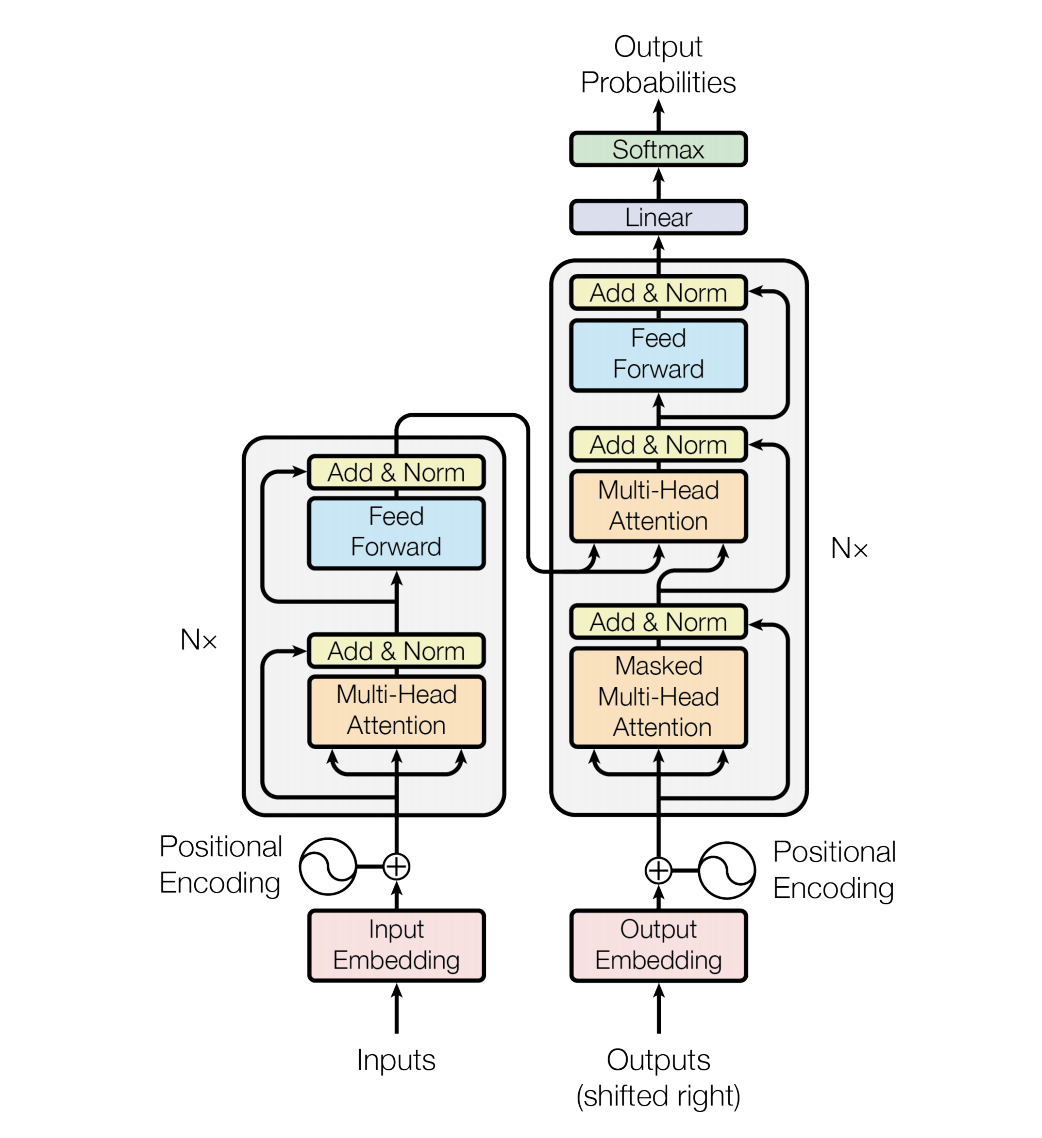
\includegraphics[height=0.5\textheight]{img/transformer}
        \caption[Original Transformer Architecture]{\textbf{Original Transformer Architecture.}
        The architecture was originally conceptualized for translation between languages.
        For that effect the text to translate (input) will be fully encoded to the embedding space, added to a positional encoding, and passed through alternating layers of self-attention and \gls{MLP} feed-forward layers with \gls{ReLU} activation, with residual connections and normalization after each.
        Output is generated autoregressively (generating each output token one-by-one, and append it to outputs to generate the next one), and has an additional layer of cross-attention to the input embedding.
        \Glspl{causal} are exclusively autoregressive decoder-only models.
        % The text to translate \textit{from} is the input, and the model will autoregressively (append selected output token to the outputs to generate the next output token until the full output has been generated) generate the full output.
        Image Source: \cite{vaswani_attention_2017}
        }
        \label{fig:transformer}
    \end{centering}
\end{figure}

% \begin{figure}[!htbp]
%     \begin{centering}
%         \subfloat[Runtime in minutes for correcting 25kb Matrix]
%         {\includegraphics[scale=0.9]{figures/results/runtime_25}} \\
%         % \caption[Correction time of 25kb]
%         % {\textbf{Runtime in minutes} for correcting the 25kb matrix.}
%         \subfloat[Runtime in minutes for correcting 50kb Matrix]
%         {\includegraphics[scale=0.9]{figures/results/runtime_50}}
%         \caption[Algorithm Runtimes]
%         {\textbf{Algorithm Runtimes} for correcting the different matrices. It
%         remains an open question why the difference between KR and RUST stays the
%         same, even though both ICE and RUST double their computation time. Smaller
%         is better.}
%         \label{fig:transformer}
%     \end{centering}
% \end{figure}


All modern language models are based on what Google introduced as the transformer architecture \cite{vaswani_attention_2017} in 2017, see the caption in \figref{transformer} for a more detailed description. \todo{actually include part on encoder and decoder in text here}
This new transformer architecture quickly established itself by outperforming other architectures available at the time with a fraction of the training cost.
An Encoder-Only transformer architecture, specifically \gls{BERT} \cite{devlin_bert_2018} set a new \gls{SOTA} for all \gls{NLP} benchmarks established at the time.

In 2019 \gls{OpenAI} introduced \gls{GPT2} \cite{radford_language_2019}, a very straightforward transformer architecture but scaled up more than previous models. \gls{GPT2} mainly demonstrated that bigger \glspl{LM} get more capable in general.
The biggest \gls{GPT2} variant had 1.5 billion parameters, which is 15x more parameters than the biggest \gls{BERT} variant had.
Others introduced models with similar parameter counts and capabilities.
\todo{figure out final main point I want to make}
% Along with significantly increasing capability in \acrlong{NLP}, these models enabled more sophisticated requests for data extraction.

% main difference to before: enabled more context compared to LSTM-based attention stuff (andscaling)

\subsection{Large Language Models}\label{sub:llm}
Models with more than a few billion parameters became generally referred to as a \acrlong{LLM}. \gls{GPT3}, the first such model with 176 billion parameters was introduced by \gls{OpenAI} in 2020 \cite{brown_language_2020}.
\glspl{LLM} differ from previous models in both parameter count (usually many billions) and substantial advances in general capability.
These models tend to have smaller siblings of the same architecture with fewer parameters, commonly in th steps of 7 billion, 13 billion, 30 billion, and 70 billion, though availability and exact parameter count varies.
Other Organisations trained \glspl{LLM} of this generation as well, some of them open-source, which demonstrated similar capabilities.
The most well-known models of this wave were \gls{bloom} and \gls{opt} (throughout 2022).

Fine-tuning \gls{GPT3} with 100 manual and 500 partially augmented examples of data extraction
created the most sophisticated pipeline for information extraction yet
\cite{dunn_structured_2022}. Most of our work will be similar to theirs. However,
Chinchilla \cite{hoffmann_training_2022} and CoTR \cite{zhang_multimodal_2023}
demonstrated that while achieving impressive capability, such large models are
substantially overparametrized and undertrained. Additionally, while the
results are state-of-the-art, GPT3 is only accessible through the API of
OpenAI, a for-profit company. This considerably limits access to model
internals.

Our work differs from \cite{dunn_structured_2022} by addressing these two
caveats. Instead of GPT3, we use a similarly capable open-source model called
OPT \cite{zhang_opt_2022}. Self-hosting enables us to do deep introspection
necessary for state-of-the-art prompt engineering and gives us the required
freedom to attempt distillation \cite{sun_patient_2019}, which addresses
overparametrization. Distillation promises substantial model parameter
reduction with little loss in accuracy (50x parameter reduction while keeping
95\% accuracy), and has been confirmed to have similar compression characteristics
for other large language models.
\todo{rewrite section on LLMs}

\subsection{The Modern Transformer Architecture}\label{sub:modern}

\todo{show picture of modern architecture and the changes made to it}

RoPE \cite{su_roformer_2022},
Grouped Query Attention \cite{ainslie_gqa_2023},
normalizing before not after individual layers
more heads
positional to each layer
etc

\section{Training Methods}\label{sec:training}
for main training usually crossentropy loss on text, decent batchsizes, large scale distributed.
\subsection{Pretraining}

\subsection{Fine-Tuning on Instructions}

\subsection{RLHF}

\section{Language Models Used}\label{sec:models}
\todo{figure out basic parameters (e.g. release date) of models used}
\todo{list all models used, their sizes, and short background descriptions}
In this Section, we introduce the models used or considered for the benchmark.

\subsection{Criteria}\label{sub:criteria}
\begin{itemize}
    \item Open-Source
    \item 7 billion parameters or more
    \item easily accessible
\end{itemize}

\subsection{OPT, Bloom}\label{sub:opt}
\todo{find third model close to OPT/bloom I was considering using}
Bloom \cite{workshop_bloom_2022}
OPT \cite{zhang_opt_2022}

more Capable: PaLM, but not open source

Originally planned to use them, but then LLaMa got released
\subsection{LLaMa}\label{sub:llama}
from meta
LLaMa \cite{touvron_llama_2023}
\subsection{Alpaca}\label{sub:alpaca}
stanford-fine-tuned instruct variant, 
\subsection{Vicuna}\label{sub:vicuna}
from meta, official llama instruct variant
\subsection{LLaMa 2}\label{sub:llama2}
from meta
\subsection{Falcon}\label{sub:falcon}
from some UAE thing

\subsection{Final List}\label{sub:list}
\begin{itemize}
    \item 
\end{itemize}


% \begin{itemize}
%     \item Attention before transformers \url{https://jalammar.github.io/visualizing-neural-machine-translation-mechanics-of-seq2seq-models-with-attention/}
%     \item Let's build GPT: from scratch, in code, spelled out. \url{https://www.youtube.com/watch?v=kCc8FmEb1nY} from Andrej Karpathy
%     \item Alternative generative models: Denoising Diffusion probabilistic models
% \end{itemize}
